\section{Review of Fourier Analysis}
We will first do a first review of Fourier transform in order to have a better introduction to Laplace transform.
\begin{parag}{Fourier transform}
	\begin{definition}
	
    A Fourier transform is a function $\hat{f}: \mathbb{R} \to \mathbb{C}$ of a given function $f : \mathbb{R} \to \mathbb{C}$, whenever $f$ is well-defined, is given as:
	\begin{align*} 
		\hat{f}\left(a\right) := \frac{1}{\sqrt{2\pi}} \int_{-\infty}^{\infty} e^{-iax}f\left(x\right)dx
	\end{align*}
	\end{definition}
	The \textit{well-defined} here is a bit sloppy but it is wanted, the transform is defined when we are able to compute the integral wrote above. But if we want to be a bit more formal we will say the well-defined means where $f$ is piecewise continuous and $\int_{-\infty}^{\infty}\left|f\right|dz < \infty$ (meaning, $f \in L^{1}\left( \mathbb{R}; \mathbb{C}\right)$)
	\begin{subparag}{Remark}
	    We also note the transform as $\mathcal{F}\left[f\right]$ instead of $\hat{f}$.
	\end{subparag}
\end{parag}

\begin{parag}{Inverse Fourier transform}
	\begin{definition}{Inverse Fourier transform}
    	let $f : \mathbb{R} \to \mathbb{C}$ of a function $f : \mathbb{R} \to \mathbb{C}$, whenever $f$ is well-defined is defined as:
		\begin{align*} 
			\check{f}\left(x\right) := \frac{1}{\sqrt{2\pi}}\int_{-\infty}^{\infty}e^{iax}f\left(a\right)da
		\end{align*}
    \end{definition}
	\begin{subparag}{Remark}
		It is also noted as $\mathcal{F}^{-1}\left[f\right]$ instead of $\check{f}$
	\end{subparag}
	Under the appropriate hypothesis of $f$, it is the inverse of the Fourier transform meaning:
	\begin{align*} 
		\mathcal{F}^{-1}\left[\mathcal{F}\left[f\right]\right] = f
	\end{align*}
\end{parag}
\begin{framedremark}
In general $\hat{f}$ is complex-valued even if $f$ is real-valued. However, if $f$ is real-valued and is even ($f\left(x\right) =  f\left(-x\right) \mathspace \forall x \in \mathbb{R}$) then $\hat{f}$ is also real-valued.
\end{framedremark}



\begin{parag}{Signal of "Physical domain"}
    The Fourier transform allows us given a signals to answer the question '\textit{How much of every frequency is in the signal}' 
\end{parag}


\begin{parag}{Properties of Fourier transform}
	The Fourier transform has several properties:
	\begin{enumerate}
	    \item Linearity: $\mathcal{F}\left[\lambda f + \mu g\right] =  \lambda \mathcal{F}\left[f\right] + \mu \mathcal{F}\left[g\right] \mathspace \lambda, \mu \in \mathbb{R}$ 
	    \item Time shift: Let $g\left(x\right) = f\left(x - x_0\right)$ then 
			\begin{align*} 
				\hat{g}\left(a\right) &=  \frac{1}{\sqrt{2\pi}}\int_{-\infty}^{\infty} e^{-iax}f\left(x\right)dx \\
				&= \frac{1}{\sqrt{2\pi}}\int_{-\infty}^{\infty}e^{-iax}f\left(x - x_0\right)dx \\
				&\underbrace{=}_{y = x - x_0} \frac{1}{\sqrt{2\pi}}\int_{-\infty}^{\infty}e^{-ia\left(y + x_0\right)}f\left(y\right)dy\\
				&= \frac{e^{-ax_0}}{\sqrt{2\pi}}\int_{-\infty}^{\infty}e^{-iay}f\left(y\right)dy\\
				&= e^{-iax_0} \hat{f}\left(a\right)
			\end{align*}
		\item Frequency shift: let $g\left(x\right) =  e^{ia_0x}f\left(x\right)$ for $a_0 \in \mathbb{R}$ 
			\begin{align*} 
				\hat{g}\left(a\right) &=  \frac{1}{\sqrt{2\pi}} \int_{-\infty}^{\infty}e^{-iax}g\left(x\right)dx\\
				&= \frac{1}{\sqrt{2\pi}}\int_{-\infty}^{\infty}e^{-iax}e^{ia_0x}f\left(x\right)dx \\
				&=  \frac{1}{\sqrt{2\pi}} \int_{-\infty}^{\infty} e^{-\left(a - a_0\right)x}f\left(x\right)dx =  \hat{f}\left(a - a_0\right)
			\end{align*}
			This can be seen as an '\textit{inverse}' of the second property
		\item Rescaling / Dilation. Let $g\left(x\right) = f\left(\lambda x\right)$ where $\lambda \in \mathbb{R}\setminus \left\{0\right\}$
			\begin{align*} 
				\hat{g}\left(a\right) = \frac{1}{\sqrt{2\pi}} \int_{-\infty}^{\infty}e^{-ax}f\left(\lambda x\right)dx
			\end{align*}
			To recover $\hat{f}$ we want to substitute $y =  \lambda x$. However we have to be careful about this substitution -- we have two cases, $\lambda$ positive or negative. When $\lambda$ is negative, it flips the orientation of the real line
			\begin{itemize}
			    \item If $\lambda > 0$ we get $\int_{-\infty}^{\infty} \cdots \frac{1}{\lambda}dy$
			    \item If $\lambda < 0$ we get $\int_{\infty}^{-\infty}\frac{1}{\lambda}dy = -\int_{-\infty}^{\infty}\cdots \frac{1}{\lambda}dy$ By merging the minus with the $\lambda$ we get that this is equal to $= \int_{-\infty}^{\infty} \cdots \frac{1}{\left|\lambda\right|}dy$
			\end{itemize}
			In both cases we have:
			 \begin{align*} 
				 \hat{g}\left(a\right) &= \frac{1}{\sqrt{2\pi}} \int_{-\infty}^{\infty}e^{-ia\frac{y}{\lambda}} f\left(y\right)\frac{1}{\left|\lambda\right|} dy \\
				 &= \frac{1}{\left|\lambda\right|} \frac{1}{\sqrt{2\pi}} \int_{-\infty}^{\infty}e^{-ia\frac{y}{\lambda}}f\left(y\right)dy\\
				 &= \frac{1}{\left|\lambda\right|} \hat{f}\left(\frac{a}{\lambda}\right)
			 \end{align*}
	\end{enumerate}
	\begin{subparag}{Remark}
	    A little interesting thing that we can see here from Analysis II is the absolute value here in the $\lambda$. The conclusion we have here is that in any case we have an absolute value. The same as when we were doing a change of variable in $\mathbb{R}^{n}$ where we took the absolute value of the determinant of the Jacobian.
	\end{subparag}
	If we were to visualize what scaling with a $\lambda$ this would give our signal something like this:
\end{parag}
\begin{figure}[h!]
\centering
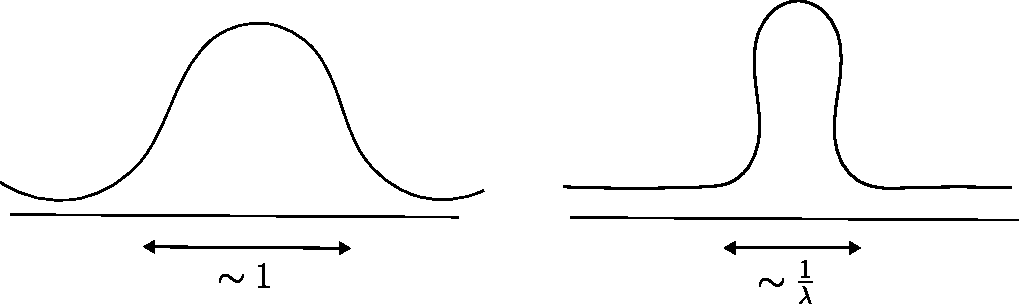
\includegraphics[width=0.7\textwidth]{figure/2026-04-16.pdf}
\caption{It misses two diagrams}
\end{figure}


\begin{parag}{Derivatives}
    Let $g\left(x\right) = f'\left(x\right)$ then 
	\begin{align*} 
		\hat{g}\left(a\right) =  ia \hat{f}\left(a\right)
	\end{align*}
	More generally 
	\begin{align*} 
		\mathcal{F}\left[f^{\left(n\right)}\right]\left(a\right) = \left(ia\right)^{n}\mathcal{F}\left[f\right]\left(a\right)
	\end{align*}
	So the Fourier transform converts differential equations with constant coefficients into algebraic equations on a frequency domain. And this is really one of the big insight, the big feature of this transform.
\end{parag}

\begin{parag}{Convolution}
    \begin{definition}
    Given $f, g : \mathbb{R} \to \mathbb{C}$, the convolution $f \ast g : \mathbb{R} \to \mathbb{C}$, whenever is well-defined is:
	\begin{align*} 
		f \ast g \left(x\right) =  \int_{-\infty}^{\infty} f\left(y\right) g\left(x - y\right)dy
	\end{align*}
    \end{definition}
	Convolution is sometime useful in order to '\textit{smooth out a function}', the German equivalent has maybe a better illustration about smoothing by blablla. But first we shall see some properties of the convolution:
	\begin{itemize}
		\item Symmetry: $f \ast g =  g\ast f$ 
	    \item Associativity: $f \ast \left(g \ast h\right) =  \left(f \ast g\right) \ast h$
	    \item Distributivity $f \ast \left(g \ast h\right) =  f \ast g + f \ast h$
	    \item $\left(f \ast g\right)' =  f' \ast g = f \ast g'$ whenever $f$ or/and are differentiable
	\end{itemize}
	The last item here is very important, it implies that $f \ast g$ is at least as smooth as the smoothest function among $f$ and $g$. Interpreted as a \textit{local average} of $f$ with weight $g$.\\
\end{parag}

\begin{parag}{Example}
    Let 
	\begin{align*} 
		g\left(x\right) = \begin{cases}
			\frac{1}{2 \epsilon} \mathspace \text{ if } x \in \left[-\epsilon, \epsilon\right]\\ 0 \text{otherwise}
		\end{cases}
	\end{align*}
	Now if we want to compute the convolution of a function $f$:
	\begin{align*} 
		f \ast g \left(x\right) &=  \int_{-\infty}^{\infty} f\left(y\right) g\left(x - y\right) dy \\
		&= \frac{1}{2\epsilon}\int_{x - \epsilon}^{x + \epsilon} f\left(y\right)dy
	\end{align*}
	So $f \ast g$ is really the local average of $f$. Note as $\epsilon \to 0$ we have $f \ast g \left(x\right) \to f\left(x\right)$ when $f$ is continuous at $x$. 
\end{parag}




\begin{parag}{Fourier transform as convolution}
    Let $f , g: \mathbb{R} \to \mathbb{C}$ then:
	\begin{align*} 
		\mathcal{F} \left[f \ast g\right] = \sqrt{2\pi} \mathcal{F}\left[f\right] \mathcal{F}\left[g\right]
	\end{align*}
	So the Fourier transform turns convolutions into products (and vis versa). In applications, one can often express $\mathcal{F}\left[f\right]$ as a product of huwu Fourier transform, which allows us to recover $f$ by convolution.
\end{parag}
\begin{parag}{Gaussian function}
    Now let us see the last property. If $f\left(x\right) = e^{\frac{-x^2}{2}}$ then the Fourier transform is:
	\begin{align*} 
		\hat{f}\left(a\right) =  e^{-\frac{a^2}{2}}
	\end{align*}
	Will be shown in the exercices, but for the sake of completeness
\end{parag}

\begin{parag}{Plancherel's Theorem}
    \begin{theoreme}
    \begin{align*}
		\int_{-\infty}^{\infty} \left|f\left(x\right)\right|^2 dx =  \int_{-\infty}^{\infty} \left|\hat{f}\left(a\right)\right|^2 da
	\end{align*}
    \end{theoreme}
\end{parag}


Okay this is nice but Fourier transform is about real function (as we have done them in Analysis III), how does complex analysis enter in the computation of Fourier transform?

\begin{parag}{Example}
    Let $f\left(x\right) = \frac{1}{1 + x^2}$ then 
	\begin{align*} 
		\hat{f}\left(a\right) = \frac{1}{\sqrt{2\pi}} \int_{-\infty}^{\infty}e^{-iax}\frac{1}{1 + x^2}dx
	\end{align*}
	we can compute this using then the residue theorem!!!!! Let $a \leq 0$. And set 
	\begin{align*} 
		f\left(z\right) = \frac{e^{-iaz}}{1 + z^2} = \frac{e^{-iaz}}{\left(z - i\right)\left(z + i\right)}
	\end{align*}
	Then in this situation, we will do the same as what we did in the previous section. Decompose the integral with a big part of the real axis, from $-R$ to $R$ and close using the half circle. In our case we will choose the upper half circle, the reason is that the goal of this is that when $R \to \infty$ the contribution this half circle has to vanish.\\
	$ $\\
	Since $a \leq 0$, when $z \in \left\{\left|z\right| =  R\right\} \cap \left\{\text{Im }z > 0\right\}$ The function $f$ decays exponentially as $R \to \infty$.
\end{parag}
\begin{figure}[h!]
\centering
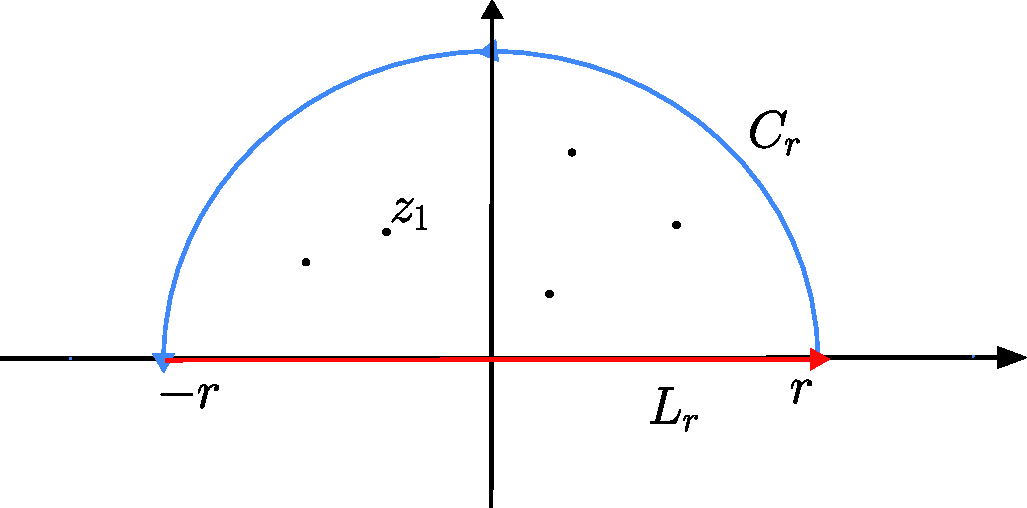
\includegraphics[width=0.6\textwidth]{figure/2026-04-04.pdf}
\caption{I am using a previous figure so don't mind the $z$ in this}
\end{figure}

\begin{parag}{ $ $}
    From previous calculations in class, 
	\begin{align*} 
		\int_{-\infty}^{\infty} f\left(x\right) dx =  2\pi i \text{Res}_i \left(f\right)
	\end{align*}
	And we can check quite easily that $i$ is a pole of order $1$, we can therefore compute the residue using the limit:
	\begin{align*} 
		&= 2\pi i \lim_{z \to i} \left(\left(z - i\right)f\left(z\right)\right)\\
		&= 2\pi i \frac{e^{a}}{2i} = \pi e^{-\left|a\right|}
	\end{align*}
	The reason of $-\left|a\right|$ is to suggest that the exponent is negative.\\
	$ $\\
	So for $a \leq 0$, we have that the transform is given as
	\begin{align*} 
		\mathcal{F}\left[\frac{1}{1 + x^2}\right] \left(a\right) = \sqrt{\frac{\pi}{2}}e^{-\left|a\right|}
	\end{align*}
	Using similar calculation for $a > 0$ by considering the semi-circle in the lower half plane we will get the same result.
	\begin{subparag}{Remark}
	    The principle is that in order to close the circle we choose the half circle depending on whether or not $a > 0$.
	\end{subparag}
\end{parag}



\section{Laplace Analysis}
The Fourier transform is made in order to computed for signals on $ \mathbb{R}$. On the other hand the Laplace transform is made in order to compute signals defined on $ \mathbb{R}_{+}$. Both transform differential equation into algebraic equation. The reason on why Laplace transform even is a thing (because we could think that every function defined for Laplace transform can be translated on $ \mathbb{R}$ (e.g., setting $f\left(x\right) = 0 \forall x < 0$))? The reason for this is \important{convergence}.

\begin{definition}
 	Let $f: \mathbb{R}_+ \to \mathbb{C}$. When well-defined, the \important{Laplace transform} of $f$ at $z \in \mathbb{C}$ is given as:
	\begin{align*} 
		\mathcal{L}\left[f\right] \left(z\right) := \int_{0}^{\infty}f\left(t\right)e^{-zt}dt
	\end{align*}
\end{definition}
Sometimes Laplace transform of functions are written by capital letters



\subsection{Convergence criteria}
Of course the above integral is well-defined if $\int_{-\infty}^{\infty}\left|f\left(t\right)\right|\left|e^{-zt}\right|dt < \infty$.\\
$ $\\
Assume that there is a $\gamma_0 \in \mathbb{R}$ s.t. 
\begin{align*} 
	\int_{0}^{\infty}\left|f\left(t\right)\right|e^{-\gamma_0 t} dt < \infty
\end{align*}
What we are claiming is that this condition is sufficient in order to the Laplace transform to be defined. Naively this means that $\left|f\left(t\right)\right| < e^{\gamma_0 t}$ as $t \to \infty$\\
$ $\\
Using the Cauchy-Schwartz inequality:
\begin{align*} 
	\left|\mathcal{L}[f]\left(z\right)\right| &\leq \int_{0}^{\infty} \left|f\left(t\right)\right|\left|e^{-zt}\right|dt\\
	&= \int_{o}^{\infty}\left|f\left(t\right)\right|\left|e^{- \text{Re }z t}\right|\underbrace{\left|e^{- \text{Im }z t i}\right|}_{= 1}dt\\
	&= \int_{0}^{\infty}\left|f\left(t\right)\right|e^{-\text{Re }z t}dt\\
	&\leq \int_{0}^{\infty} \left|f\left(t\right)\right|e^{-\gamma_0 t}dt < \infty
\end{align*}
This mean that if such a $\gamma_0$ exists, $\mathcal{L}\left[f\right]\left(z\right)$ is defined at least for $z \in \left\{z \in \mathbb{C} : \text{Re }z > \gamma_0\right\}$. Such a $\gamma_0$ has a name:

\begin{definition}{abscissa of convergence}
	A $\gamma_0 \in \mathbb{R}$ such that $\mathcal{L}\left[f\right]\left(z\right)$ is well defined at least on $\left\{\text{Re} > \gamma_0\right\}$ is called abscissa of convergence.
\end{definition}







\begin{parag}{Derivative}
    If $f\left(t\right) =  0$ for $t \geq M$ and $f$ is piecewise continuous then the Laplace transform can be computed as:
	\begin{align*} 
		\int_{0}^{\infty}\left|f\left(t\right)\right|e^{-\gamma_0 t}dt =  \int_{0}^{M}\left|f\left(t\right)\right|e^{-\gamma_0 t}dt < \infty \mathspace \mathspace \forall \gamma_0 \in \mathbb{R}
	\end{align*}
	In this case, $\mathcal{L}\left[f\right]\left(z\right)$ is defined for all $z \in \mathbb{C}$\\
	$ $\\
	Let us have another example. Let $\gamma_0$ be an abscissa of convergence. Then $\mathcal{L}\left[f\right]$ is holomorphic.

On $\left\{\text{Re } > \gamma_0\right\}$. Set $F\left(z\right) =  \mathcal{L}\left[f\right]\left(z\right)$. Then:
\begin{align*} 
	\frac{d}{dz} F\left(z\right) &= \frac{d }{dz} \int_{0}^{\infty}f\left(t\right)e^{-zt}dt\\
	&= \int_{0}^{\infty}f\left(t\right)\left(-t\right)e^{-zt} =  -\mathcal{L}\left[tf\left(t\right)\right]\left(z\right)
\end{align*}
	In short, 
	\begin{align*} 
		\mathcal{L}\left[f\left(t\right)\right]' =  - \mathcal{L}\left[tf\left(t\right)\right]
	\end{align*}
	\begin{subparag}{Remark}
	    Here we have implicitly used that if $\gamma_0 \in \mathbb{R}$ is an abscissa of convergence for $\mathcal{L}\left[f\left(t\right)\right]$ so it is for $\mathcal{L}\left[tf\left(t\right)\right]$.
	\end{subparag}
\end{parag}



\begin{parag}{Example}
    Let $f\left(z\right) = 1$. Then for every $\gamma_0 > 0$
	\begin{align*} 
		\int_{0}^{\infty}\left|f\left(t\right)\right|e^{-\gamma_0 t}dt =  \int_{0}^{\infty}e^{-\gamma_0 t}dt = \frac{1}{\gamma_0} < \infty
	\end{align*}
	So any $\gamma_0 > 0$ is an abscissa of convergence, hence $\mathcal{L}\left[f\right]\left(z\right)$ is defined for $z \in \left\{\text{Re } > 0\right\}$. Moreover:
	\begin{align*} 
		\mathcal{L}[f]\left(z\right) = \int_{0}^{\infty}e^{-zt} dt \underbrace{= }_{z \neq 0}\left[\frac{e^{-zt}}{-z}\right]_{0}^{\infty}
	\end{align*}
	\begin{subparag}{Note}
	    \begin{align*} 
			\lim_{t \to \infty} e^{-zt} =  0
		\end{align*}
		If $\text{Re }z > 0$ since:
		\begin{align*} 
			\left|e^{-zt}\right| = \underbrace{\left|e^{- \text{Re }zt}\right|}_{\to 0}\underbrace{\left|e^{- \text{Im }z ti}\right|}_{= 1}
		\end{align*}
		As $t \to \infty$
	\end{subparag}
	Therefore, $\mathcal{L}\left[1\right]\left(z\right) = \frac{1}{z}$
\end{parag}


